\documentclass{article}%
\usepackage[T1]{fontenc}%
\usepackage[utf8]{inputenc}%
\usepackage{lmodern}%
\usepackage{textcomp}%
\usepackage{lastpage}%
\usepackage{geometry}%
\geometry{margin=1in}%
\usepackage[utf8]{inputenc}%
\usepackage[titletoc,title]{appendix}%
\usepackage{graphicx,float}%
\usepackage{ragged2e}%
%
\title{\textbf{RELATÓRIO TÉCNICO DE SAÚDE PÚBLICA - INFLUENZA}}%
%
\begin{document}%
\normalsize%
\maketitle%
\section{Análise}%
\label{sec:Anlise}%
\subsection{Geral}%
\label{subsec:Geral}%
A análise dos dados revela uma redução significativa no número total de casos de SRAG no Brasil ao longo dos anos, passando de 1.716.860 em 2021 para 284.138 em 2023, e mantendo{-}se em níveis semelhantes em 2024 e 2025. Apesar dessa diminuição, o número de internações em UTI também caiu de 502.428 em 2021 para 76.372 em 2023, indicando uma melhora na gravidade dos casos ou na eficácia das intervenções. No entanto, o aumento na vacinação, que atingiu mais de 40.000 doses em 2025, sugere uma estratégia contínua de controle, embora os dados de mortalidade também tenham apresentado uma redução expressiva, de 436.547 óbitos em 2021 para 15.048 em 2025. Esses números indicam uma tendência de diminuição na incidência e na gravidade da crise de SRAG, embora a vigilância e a vacinação permaneçam essenciais para evitar possíveis recrudescimentos.\newline%
%
A taxa de mortalidade por SRAG no Brasil apresentou uma redução significativa entre 2021 e 2025, passando de 25,4\% em 2021 (436.547 óbitos de 1.716.860 casos) para aproximadamente 5,3\% em 2025 (15.048 óbitos de 229.300 casos). Essa diminuição pode estar relacionada ao aumento na taxa de vacinação, que cresceu de 56.918 vacinados em 2021 para 40.571 em 2025, além de melhorias nos cuidados médicos e na gestão da crise. Apesar da redução na mortalidade, o número de casos ainda é elevado, indicando a necessidade de continuidade de estratégias de prevenção e controle.\newline%
%
A taxa de ocupação de UTIs por pacientes com SRAG apresentou uma redução significativa ao longo dos anos, passando de 502.428 internados em 2021 para 59.256 em 2025, indicando uma melhora na capacidade hospitalar e possível impacto das campanhas de vacinação. Essa diminuição coincide com a redução do número de óbitos, que caiu de 436.547 em 2021 para 15.048 em 2025, refletindo uma possível melhora no manejo clínico e na prevenção da doença. No entanto, a persistência de internações e óbitos evidencia a necessidade de continuidade de ações de controle e monitoramento da crise de SRAG no Brasil.\newline%
%
A taxa de vacinação contra COVID{-}19 e gripe no Brasil apresentou crescimento ao longo dos anos, passando de 56.918 vacinados em 2021 para 40.571 em 2025, indicando esforços contínuos de imunização. Apesar do aumento na cobertura vacinal, os dados de casos de SRAG e óbitos ainda demonstram uma redução significativa, com o total de casos caindo de 1.716.860 em 2021 para 268.491 em 2024 e óbitos reduzidos de 436.547 para 15.048 no mesmo período, sugerindo que a vacinação tem contribuído para o controle da crise, embora a persistência de casos e óbitos ressalte a necessidade de manutenção e ampliação das estratégias de vacinação e de outras medidas de saúde pública.\newline%

%
\subsection{Relação Mensal e Anual}%
\label{subsec:RelaoMensaleAnual}%
Nos últimos 30 dias, o total de casos de SRAG apresentou variações, com picos notáveis em dias 1, 8, 15, 22 e 29, indicando possíveis surtos ou aumento na transmissão. Apesar de alguns dias apresentarem redução no número de casos, a tendência geral demonstra uma oscilação, reforçando a necessidade de monitoramento contínuo e ações de controle. A análise sugere que, embora haja momentos de diminuição, a persistência de casos em níveis elevados evidencia a importância de fortalecer estratégias de prevenção, diagnóstico e tratamento para conter a crise de SRAG no país.\newline%
%
Ao longo dos últimos 12 meses, o Brasil apresentou um aumento significativo no número de casos de SRAG, atingindo o pico em abril com 31.046 registros, seguido de uma leve redução nos meses subsequentes, embora os números permaneçam elevados. O mês de maio também apresentou alta incidência, enquanto os meses de junho a dezembro mostraram uma tendência de declínio, com o menor número de casos em dezembro (14.935). Essa variação sugere uma crise persistente, com períodos de agravamento e melhora, refletindo a necessidade de estratégias contínuas de controle e vacinação.\newline%
%


\begin{figure}[H]%
\begin{minipage}{0.45\textwidth}%
\centering%
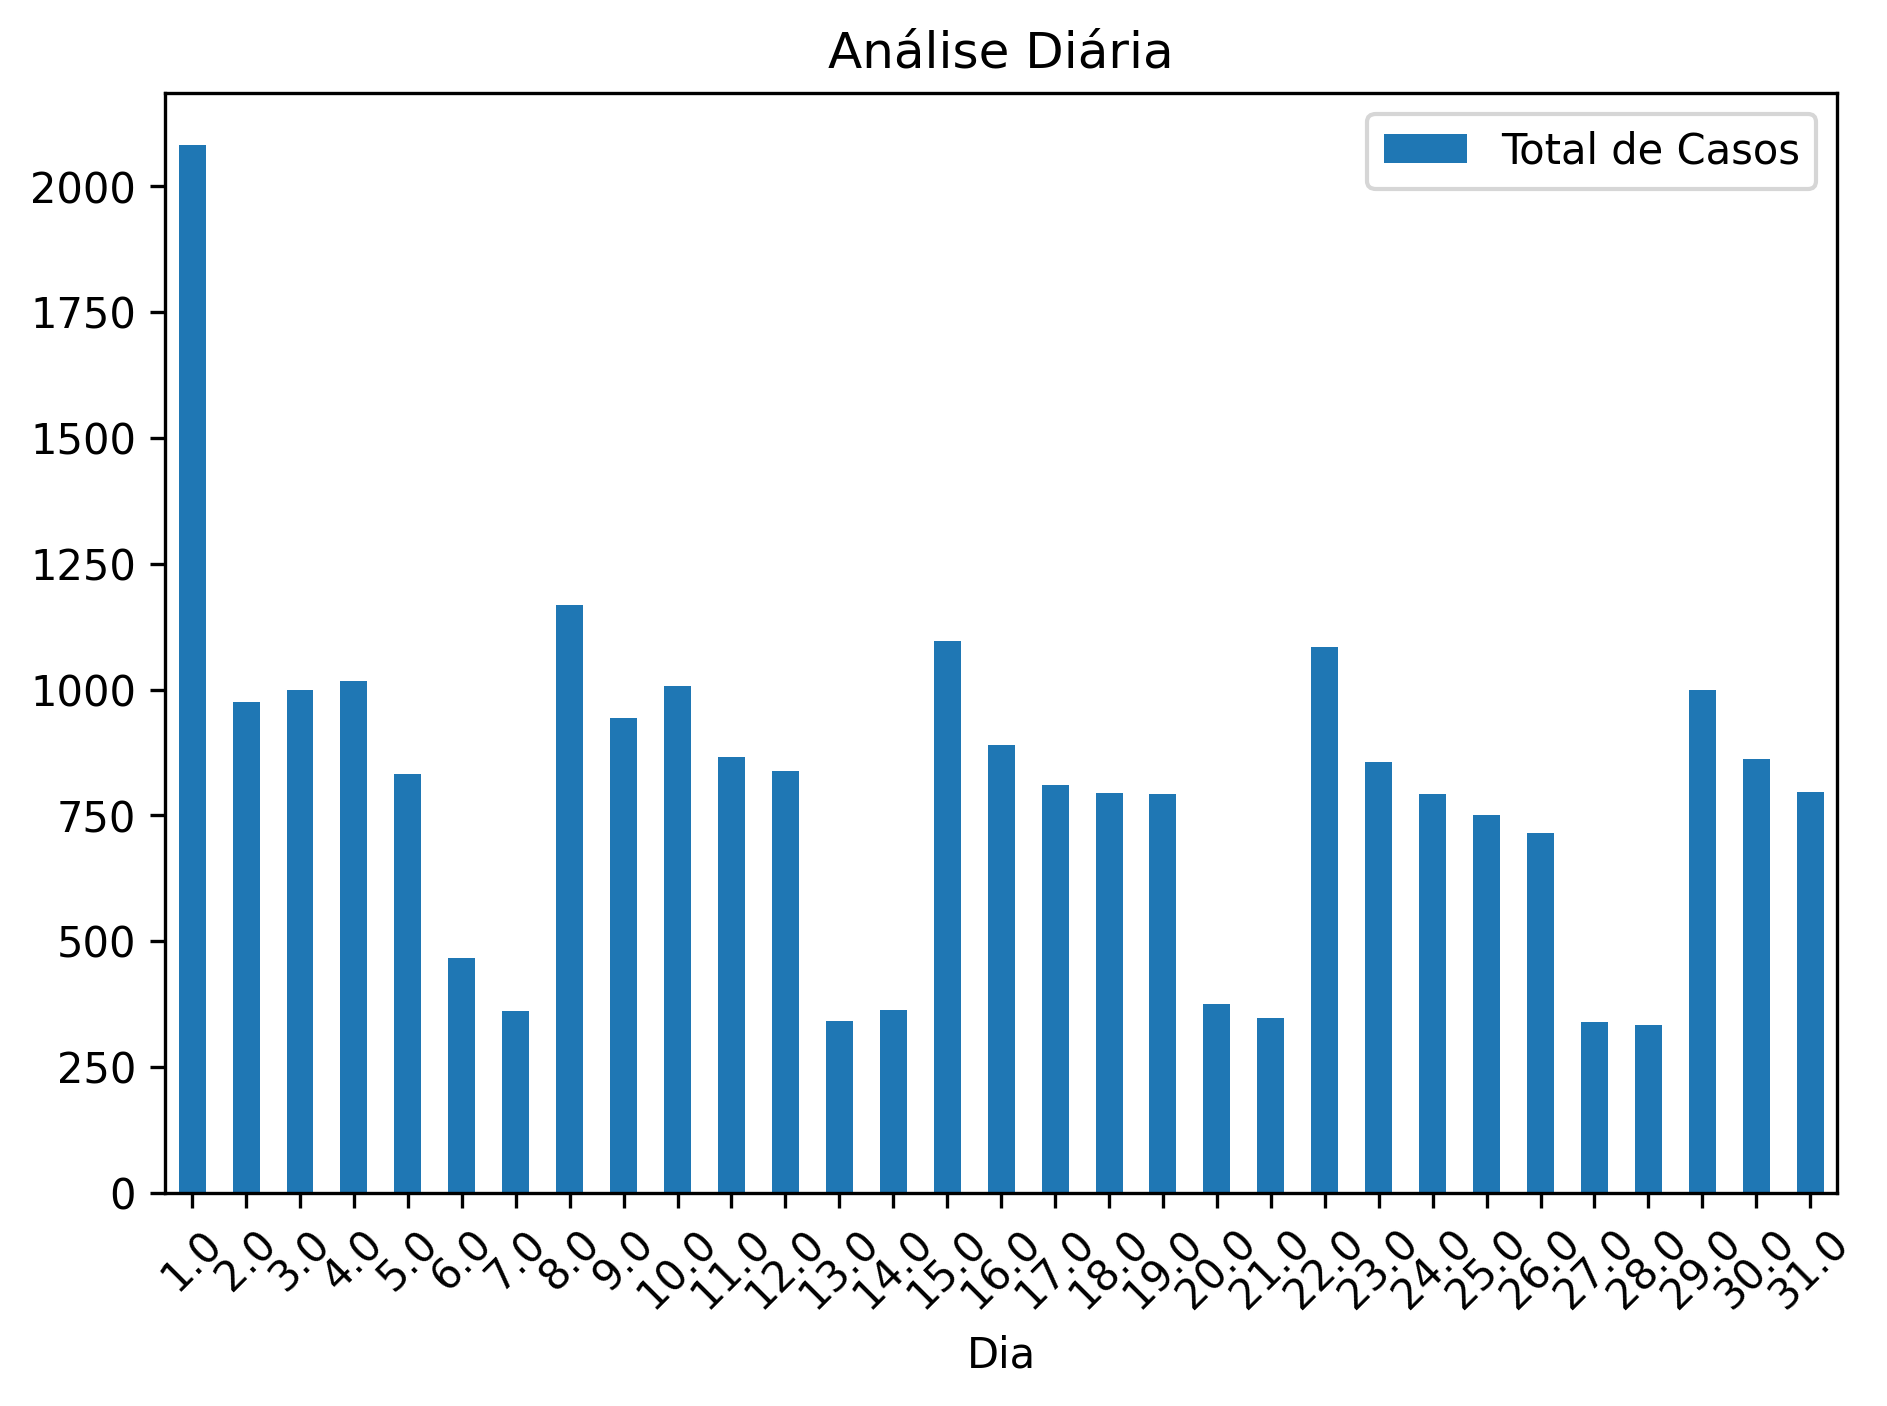
\includegraphics[width=\textwidth]{../graphics/monthly-analysis.png}%
\caption{Análise Mensal}%
\label{fig:casos-30-dias}%
\end{minipage}%
\begin{minipage}{0.45\textwidth}%
\centering%
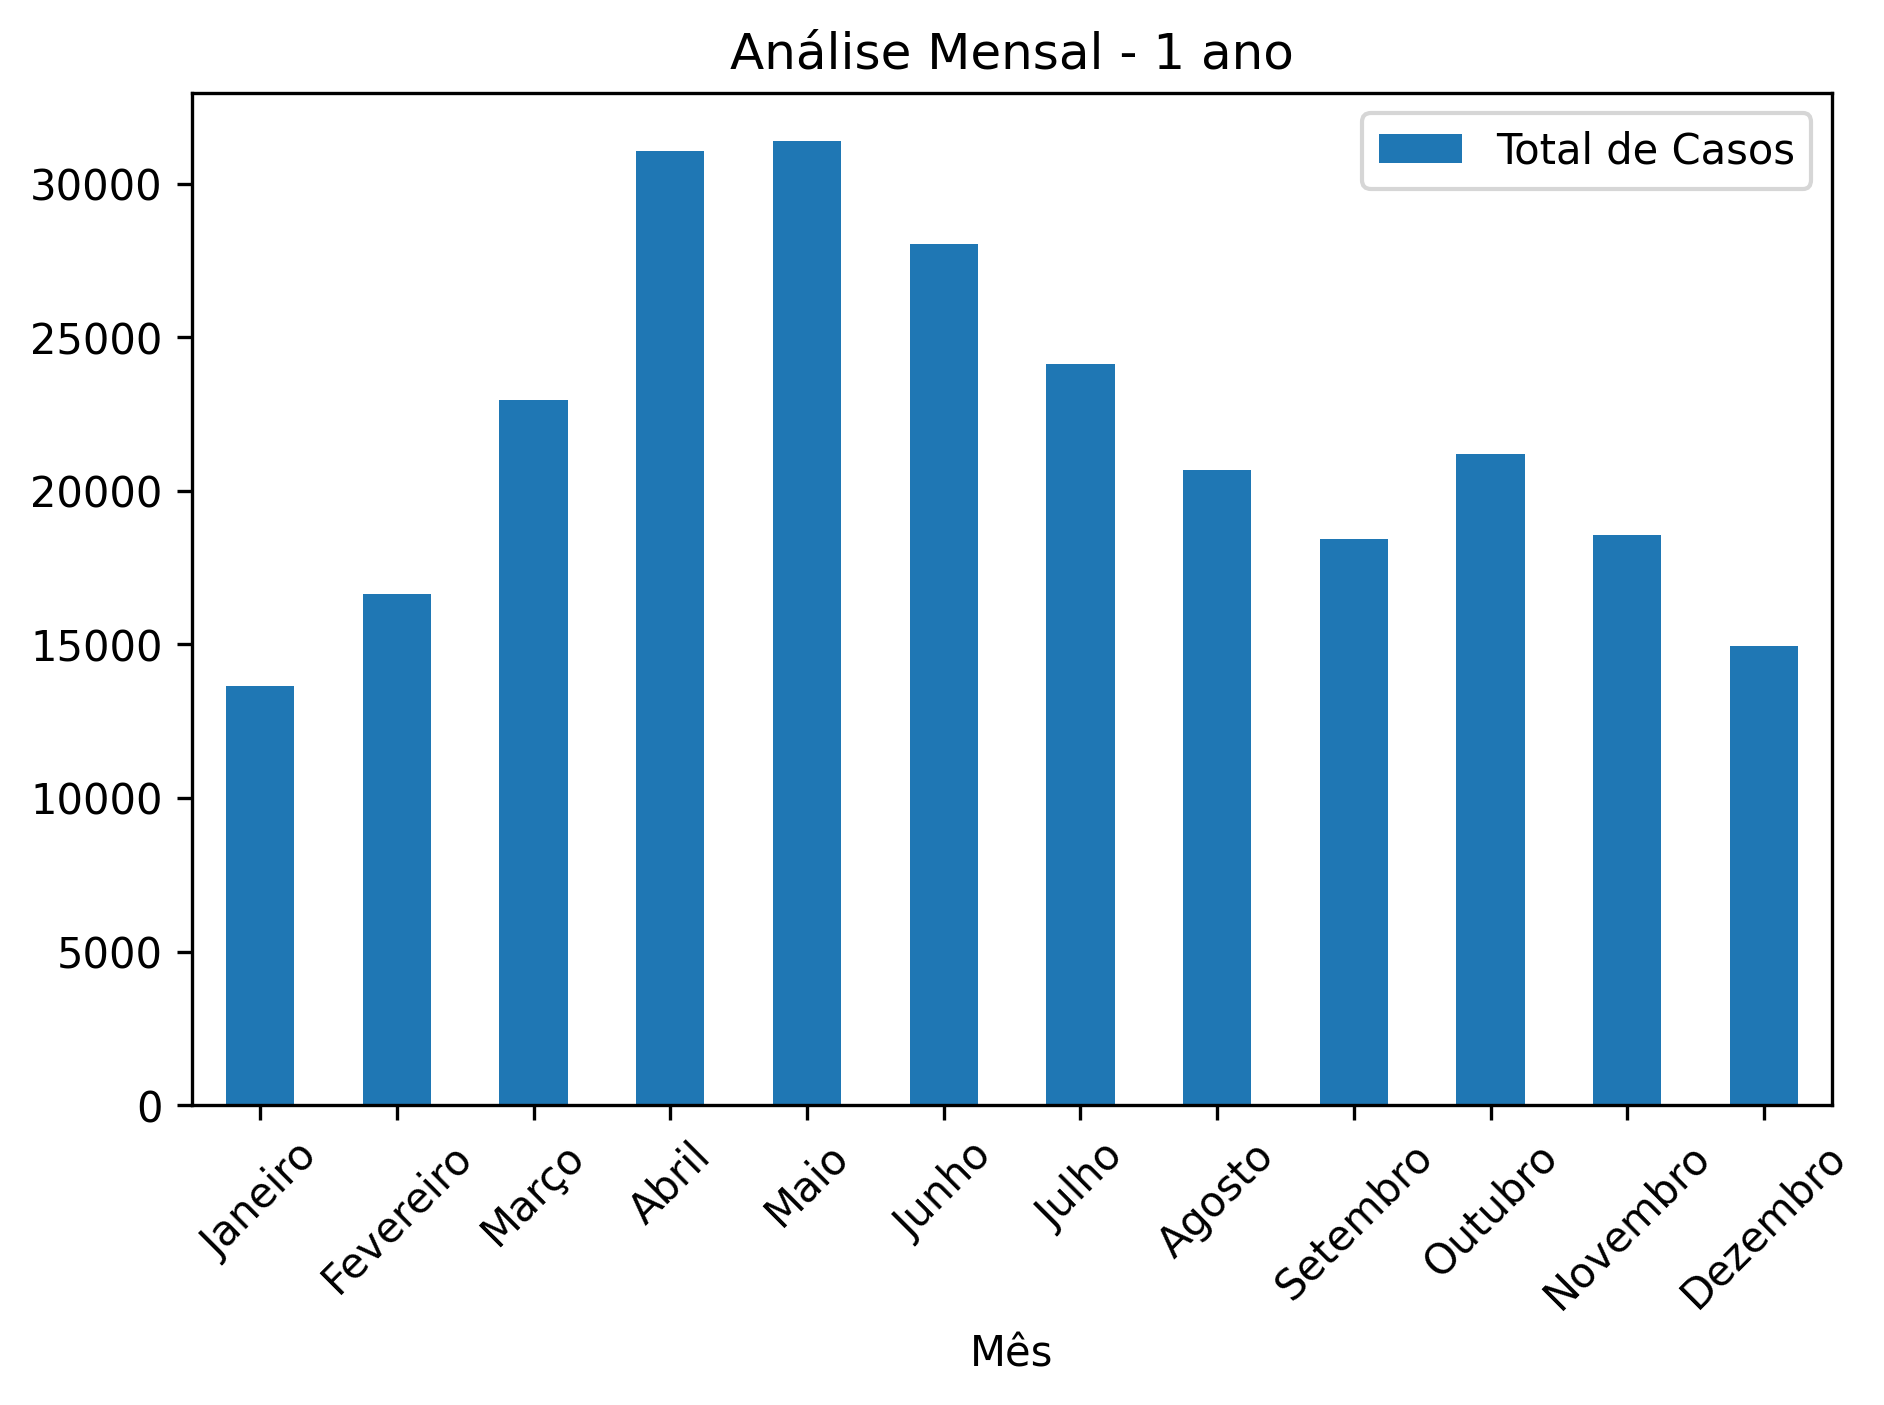
\includegraphics[width=\textwidth]{../graphics/yearly-analysis.png}%
\caption{Análise Anual}%
\label{fig:casos-12-meses}%
\end{minipage}%
\end{figure}

%
\end{document}